  
\subsection{Utilizando observaciones visuales del ambiente}

Este último experimento es sobre una configuración donde el agente 
no tiene acceso a las macro variables $\mathcal{X}$ directamente. Sin embargo recibe imágenes del estado del ambiente como observaciones. A diferencia de las
configuraciones experimentales anteriores, aquí se fijan todos los parámetros que se evaluaron antes y solo se evalúa el desempeño de los algoritmos sobre mundos deterministas y estocásticos. 

\subsubsection{Configuración experimental}

\begin{itemize}
    \item Los elementos del espacio de estados $\mathcal{S}$, son continuos.
    Las observaciones son imágenes de $84\times 84$ pixeles en un espacio de color RGB, obtenidas desde una vista cenital del ambiente como se muestra en la Figura \ref{fig:obs-example-lights}.
    
    \begin{figure}[H]
        \centering
        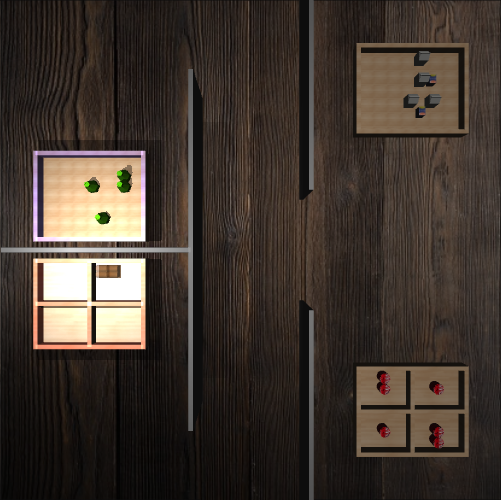
\includegraphics[scale=0.2]{Chapter5/Figs/obs_example.png}
        \caption{Ejemplo de una posible observación del agente.}
        \label{fig:obs-example-lights}
    \end{figure}
    \item Para mapear las imágenes al espacio de estados de alto nivel $\mathcal{X}$, la función $\phi$ es un clasificador multi etiqueta
    parametrizado por una red neuronal convolucional \cite{Goodfellow-et-al-2016} (CNN por sus siglas en inglés). La arquitectura de la red, de manera visual, se presenta en la Figura \ref{fig:cnn-classifier}. Al agente se le brinda el clasificador ya entrenado.
    La salida de la red son procesadores $p_i$ que
    representan la probabilidad de que la variable $x_i$ tome el valor 1, donde
    $i \in \{1, \dots, l\}$. Por simplicidad se utiliza un solo
    clasificador para los distintos experimentos. Por lo tanto, $l = 9$ y
    para los casos donde $N < 9$ entonces se suponen las variables mayores
    a $N$ como apagadas. 
    \item Se prueba sobre dos versiones del ambiente, una discreta y otra estocástica.
    \item El valor de parámetro de alteración del grafo causal correcto es
    $p_{mod} = 25$.
    \item La tasa de decremento de $\epsilon$ está controlada por el factor $\delta = 0.75$.
    \item Dado que las observaciones son imágenes, se utiliza la versión 
    del algoritmo Q-learning para estados continuos DQN. La arquitectura e hiperparámetros de entrenamiento son los mismos que los del artículo original del método DQN 
    \cite{mnih2015human}. 
\end{itemize}    
\begin{figure}[h]
    \centering
    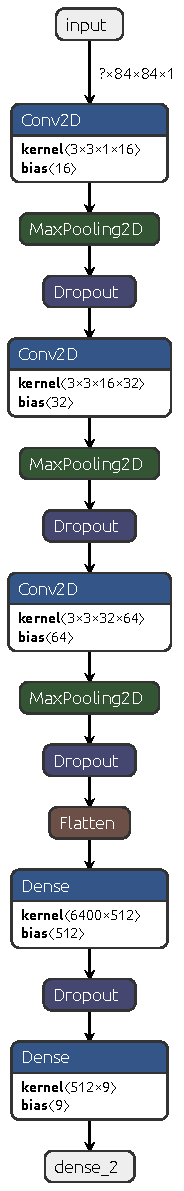
\includegraphics[scale=0.6]{Chapter5/Figs/multilabel_classifier.pdf}
    \caption{Arquitectura del clasificador multi etiqueta, $\phi$, que
    mapea observaciones visuales a un conjunto de variables
    de alto nivel.}
    \label{fig:cnn-classifier}
\end{figure}

\subsubsection{Objetivo}

Determinar si el modelo causal con variables  en otro espacio siguen conservando las propiedades
de ayudar en el aprendizaje como en los casos discretos.

\subsubsection{Hipótesis}

Si se cuenta con información de las observaciones
en un espacio más pequeño, pero donde se codifiquen
los estados en alto nivel, se puede apoyar 
al algoritmo de aprendizaje a alcanzar una recompensa
mayor en menos tiempo.

\subsubsection{Resultados}

De acuerdo con las Figuras \ref{fig:dqn-results-det} y \ref{fig:dqn-results-sto} los algoritmos que utilizan conocimiento del grafo inician con una recompensa mayor y mantienen esa medida de desempeño por encima del algoritmo DQN
sin información adicional. 

Además de las curvas de aprendizaje se realiza la prueba estadística de Welch para validar la diferencia entre los métodos usando el información extra y sin usarla. Para esto, se compara la recompensa promedio de los últimos $E = 20$ episodios
de entrenamiento sobre los $M$ experimentos. 
% Con esto, se 
% obtiene una muestra de tamaño $E$ para cada algoritmo
% y se realiza la prueba estadística de Welch. La prueba estadística se realiza comparando los algoritmos que utilizan alguna estructura causal y el algoritmo Q-learning usando una exploración a prueba y error para saber si los primeros son superiores significativamente sobre el segundo. 
En los Cuadros \ref{tab:dqn-one-to-one}, \ref{tab:dqn-one-to-many} y \ref{tab:dqn-many-to-one} se muestran
los promedios de las recompensas durante los últimos 20 episodios para los 10 experimentos.
De igual manera que en las curvas de aprendizaje se puede notar que en la mayoría de tareas el algoritmo DQN que utiliza grafo causal completo tiene una recompensa mayor que en los otros métodos. Además, en general los métodos que utilizan el grafo ya sea incorrecto o incompleto superan al método clásico de Q-learning. De acuerdo con la prueba de Welch con $p < 0.05$ existe una diferencia estadística en el desempeño de los algoritmos, excepto por algunos casos (marcados por $\dagger$ en las tablas). Estas excepciones surgen en tareas que involucran una estructura uno a uno pero la diferencia parece ser más signicativa conforme $N$ aumenta.


\clearpage
\begin{table}[]
\centering
\caption{Comparación de la recompensa promedio obtenida durante los últimos $E=20$ episodios de entrenamiento en $M=10$ experimentos en tareas con una estructura causal uno a uno.}
\label{tab:dqn-one-to-one}
\resizebox{\textwidth}{!}{%
\begin{tabular}{cclll}
\hline
Ambiente & Algoritmo & \multicolumn{3}{c}{$N$} \\ \cline{3-5} 
 &  & \multicolumn{1}{c}{5} & \multicolumn{1}{c}{7} & \multicolumn{1}{c}{9} \\ \hline
Determinista & $Q_{1}$ & $-2.3066 \pm 0.5624$ & $-4.6056 \pm 0.8990$ & $-6.7952 \pm 1.0171$ \\
 & $Q_{2}$ & $-2.1533 \pm 0.3999\dagger$ & $\mathbf{-3.6159 \pm 0.8505}$ & $\mathbf{-5.1539 \pm 0.9319}$ \\
 & $Q_{2}$ & $\mathbf{-2.0352 \pm 0.5624\dagger}$ & $-4.3386 \pm 1.0322\dagger$ & $-5.8771 \pm 0.9200$ \\
 & $Q_{4}$ & $-2.2114 \pm 0.3861\dagger$ & $-4.2858 \pm 0.6839\dagger$ & $-6.2123 \pm 1.1899\dagger$ \\ \cline{2-5} 
Estocástico & $Q_{1}$ & $-2.5178 \pm 0.9375$ & $-4.3270 \pm 0.9586$ & $-6.8949 \pm 1.6305$ \\
 & $Q_{2}$ & $-2.1234 \pm 0.5553\dagger$ & $\mathbf{-3.8835 \pm 0.9441\dagger}$ & $\mathbf{-5.9713 \pm 1.1062}$ \\
 & $Q_{2}$ & $-2.1962 \pm 0.5526\dagger$ & $-3.9167 \pm 0.8074\dagger$ & $-6.3114 \pm 1.1663\dagger$ \\
 & $Q_{4}$ & $\mathbf{-2.1131 \pm 0.5741\dagger}$ & $-3.9460 \pm 0.7128\dagger$ & $-6.1702 \pm 1.3293\dagger$ \\ \hline
\end{tabular}%
}
\end{table}

\begin{table}[]
\centering
\caption{Comparación de la recompensa promedio obtenida durante los últimos $E=20$ episodios de entrenamiento en $M=10$ experimentos en tareas con estructuras con causas comunes.}
\label{tab:dqn-one-to-many}
\resizebox{\textwidth}{!}{%
\begin{tabular}{cclll}
\hline
Ambiente & Algoritmo & \multicolumn{3}{c}{$N$} \\ \cline{3-5} 
 &  & \multicolumn{1}{c}{5} & \multicolumn{1}{c}{7} & \multicolumn{1}{c}{9} \\ \hline
Determinista & $Q_{1}$ & $-1.6061 \pm 0.7798$ & $-3.0271 \pm 0.6992$ & $-4.1675 \pm 0.9731$ \\
 & $Q_{2}$ & $\mathbf{-0.9634 \pm 0.3193}$ & $-2.3705 \pm 0.6772$ & $-3.6672 \pm 0.7790\dagger$ \\
 & $Q_{2}$ & $-1.2556 \pm 0.5663\dagger$ & $-2.4601 \pm 0.3798$ & $\mathbf{-3.6240 \pm 0.8182\dagger}$ \\
 & $Q_{4}$ & $-1.2576 \pm 0.4415\dagger$ & $\mathbf{-2.1523 \pm 0.5615}$ & $-3.7220 \pm 1.1360\dagger$ \\ \cline{2-5} 
Estocástico & $Q_{1}$ & $-1.8378 \pm 0.9002$ & $-2.9177 \pm 0.7892$ & $-4.9370 \pm 1.5714$ \\
 & $Q_{2}$ & $\mathbf{-0.9333 \pm 0.3057}$ & $\mathbf{-2.3807 \pm 0.8843\dagger}$ & $-3.4889 \pm 0.8272$ \\
 & $Q_{2}$ & $-1.2414 \pm 0.3751$ & $-2.5865 \pm 0.5136\dagger$ & $\mathbf{-3.1540 \pm 0.9259}$ \\
 & $Q_{4}$ & $-0.9427 \pm 0.4010$ & $-2.4278 \pm 0.5948$ & $-4.3030 \pm 0.9586\dagger$ \\ \hline
\end{tabular}%
}
\end{table}

\begin{table}[]
\centering
\caption{Comparación de la recompensa promedio obtenida durante los últimos $E=20$ episodios de entrenamiento en $M=10$ experimentos en tareas con estructuras subyacentes del tipo efecto común.}
\label{tab:dqn-many-to-one}
\resizebox{\textwidth}{!}{%
\begin{tabular}{cclll}
\hline
Ambiente & Algoritmo & \multicolumn{3}{c}{$N$} \\ \cline{3-5} 
 &  & \multicolumn{1}{c}{5} & \multicolumn{1}{c}{7} & \multicolumn{1}{c}{9} \\ \hline
Determinista & $Q_{1}$ & $-1.6981 \pm 0.7195$ & $-2.9280 \pm 0.8702$ & $-4.2433 \pm 1.0539$ \\
 & $Q_{2}$ & $-1.0877 \pm 0.4234$ & $\mathbf{-1.9022 \pm 0.5934}$ & $-3.3166 \pm 0.8006$ \\
 & $Q_{2}$ & $\mathbf{-1.0125 \pm 0.2740}$ & $-2.2917 \pm 0.7138$ & $\mathbf{-3.2871 \pm 0.6417}$ \\
 & $Q_{4}$ & $-1.1123 \pm 0.4488$ & $-2.2722 \pm 0.6711$ & $-3.8038 \pm 1.0237\dagger$ \\ \cline{2-5} 
Estocástico & $Q_{1}$ & $-1.4544 \pm 0.7061$ & $-3.0986 \pm 0.6664$ & $-3.9579 \pm 0.9685$ \\
 & $Q_{2}$ & $\mathbf{-0.8161 \pm 0.3058}$ & $-1.9340 \pm 0.4379$ & $\mathbf{-2.9446 \pm 0.6062}$ \\
 & $Q_{2}$ & $-0.9094 \pm 0.3591$ & $\mathbf{-1.8915 \pm 0.6378}$ & $-3.2302 \pm 0.8894$ \\
 & $Q_{4}$ & $-0.9650 \pm 0.3063$ & $-1.9705 \pm 0.6130$ & $-3.1761 \pm 0.9211$ \\ \hline
\end{tabular}%
}
\end{table}

\begin{figure}
\settoheight{\tempdima}{\includegraphics[width=.32\linewidth]{example-image-a}}%
\centering\begin{tabular}{@{}c@{ }c@{ }c@{ }c@{}}
&\textbf{Uno-a-uno} & \textbf{Causa común} & \textbf{Efecto común} \\
\rowname{$N = 5$}&
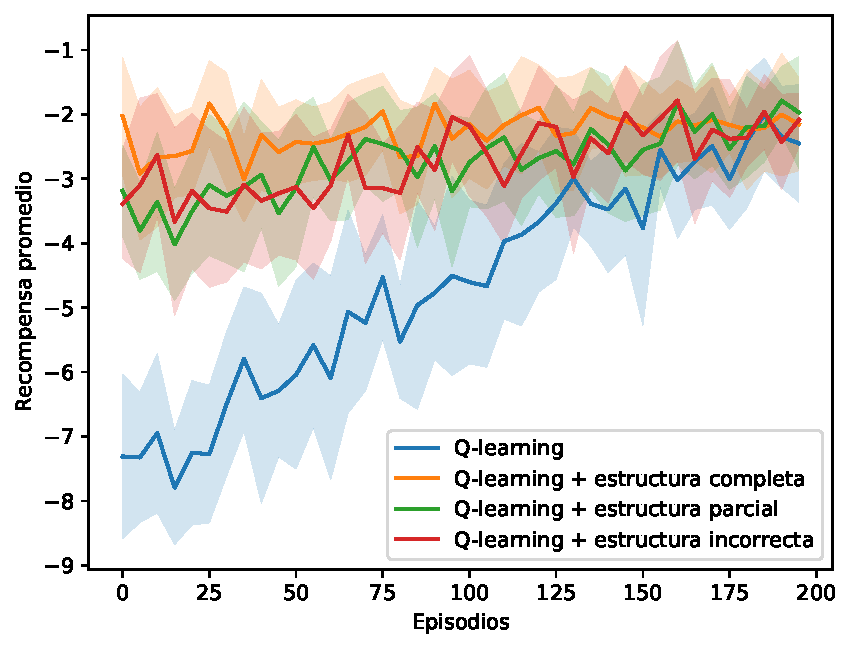
\includegraphics[width=.32\linewidth]{Chapter5/Figs/dqn/deterministic_low_025_one_to_one_N_5_experiments_10_episodes_200_eps_75.pdf}&
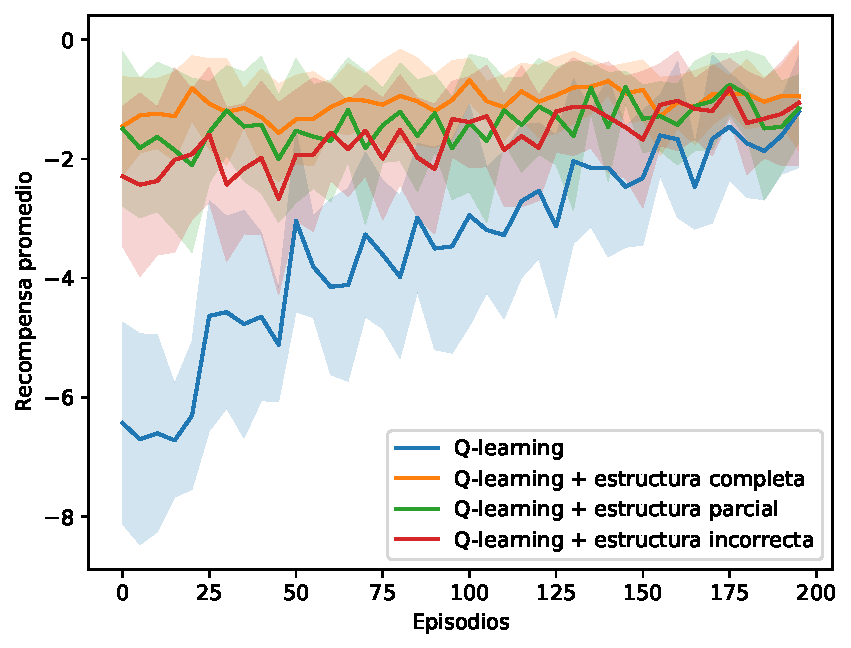
\includegraphics[width=.32\linewidth]{Chapter5/Figs/dqn/deterministic_low_025_one_to_many_N_5_experiments_10_episodes_200_eps_75.pdf}&
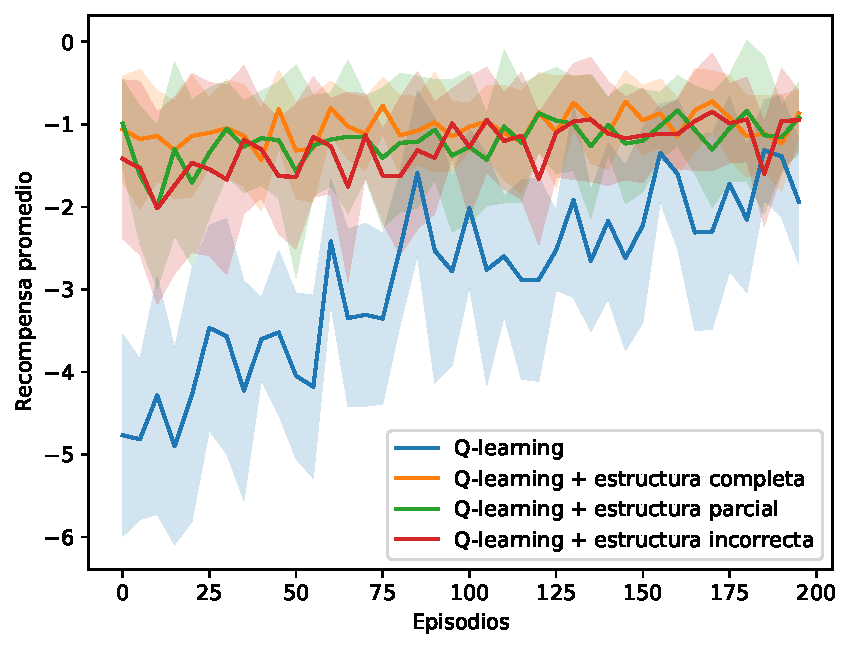
\includegraphics[width=.32\linewidth]{Chapter5/Figs/dqn/deterministic_low_025_many_to_one_N_5_experiments_10_episodes_200_eps_75.pdf}\\
\rowname{$N=7$}&
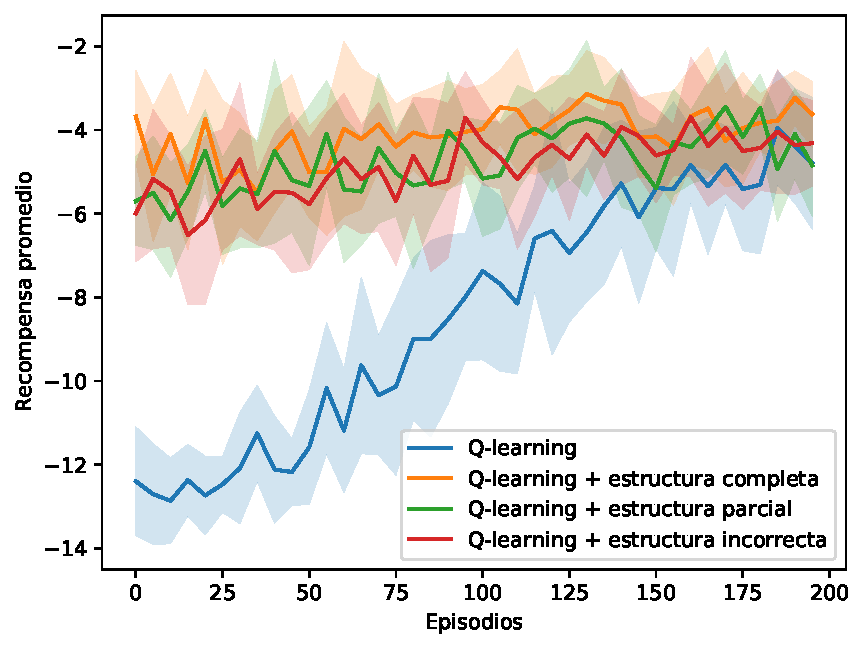
\includegraphics[width=.32\linewidth]{Chapter5/Figs/dqn/deterministic_low_025_one_to_one_N_7_experiments_10_episodes_200_eps_75.pdf}&
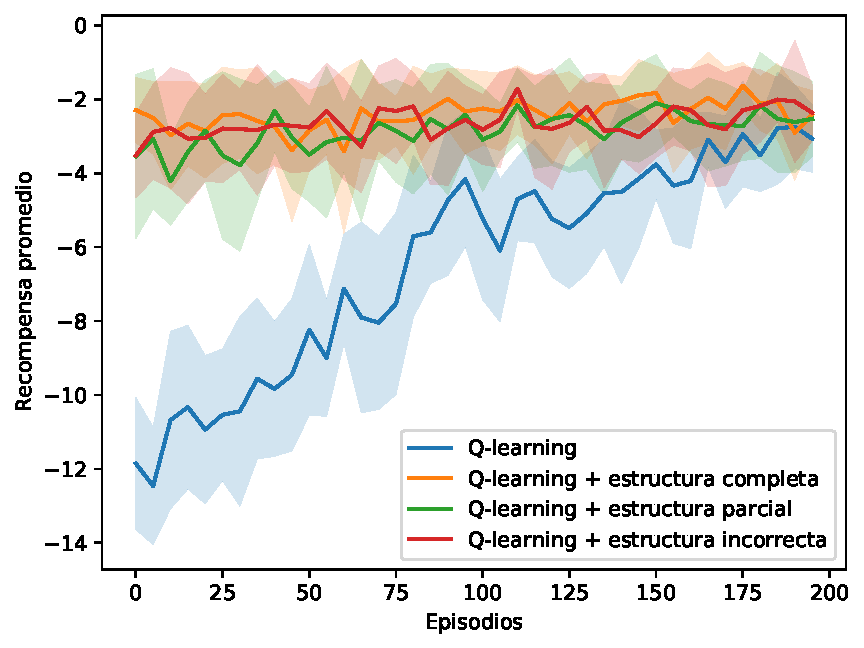
\includegraphics[width=.32\linewidth]{Chapter5/Figs/dqn/deterministic_low_025_one_to_many_N_7_experiments_10_episodes_200_eps_75.pdf}&
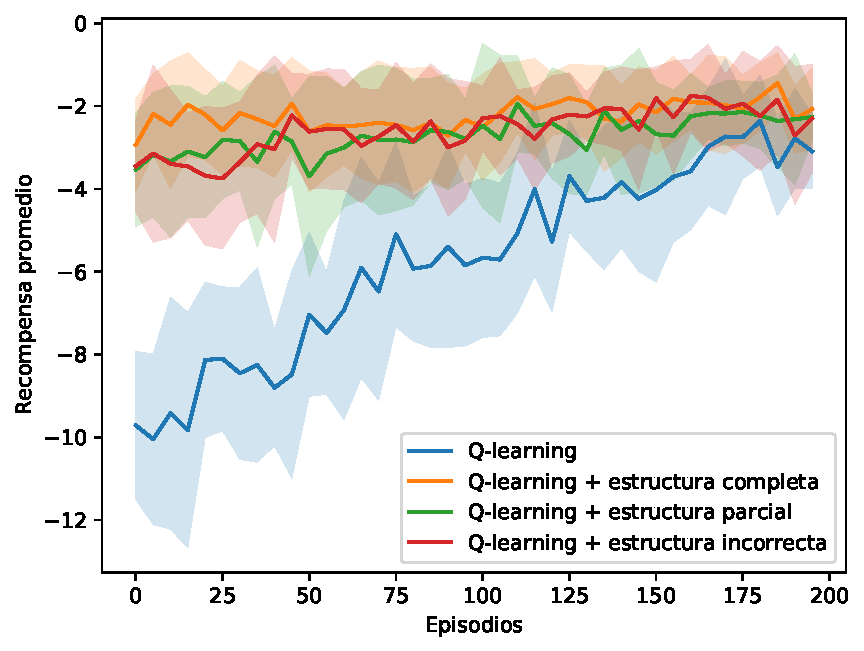
\includegraphics[width=.32\linewidth]{Chapter5/Figs/dqn/deterministic_low_025_many_to_one_N_7_experiments_10_episodes_200_eps_75.pdf}\\
\rowname{$N = 9$}&
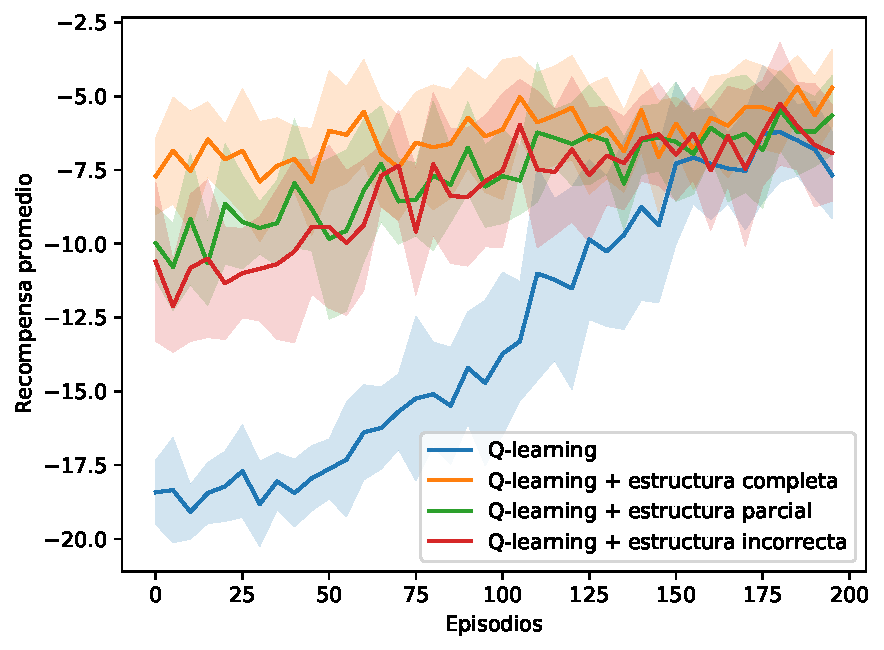
\includegraphics[width=.32\linewidth]{Chapter5/Figs/dqn/deterministic_low_025_one_to_one_N_9_experiments_10_episodes_200_eps_75.pdf}&
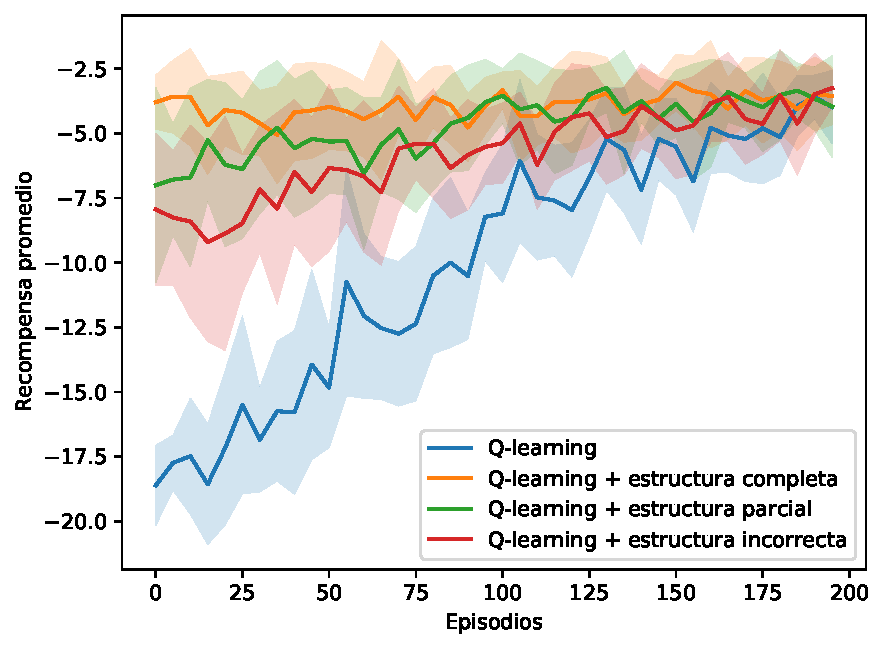
\includegraphics[width=.32\linewidth]{Chapter5/Figs/dqn/deterministic_low_025_one_to_many_N_9_experiments_10_episodes_200_eps_75.pdf}&
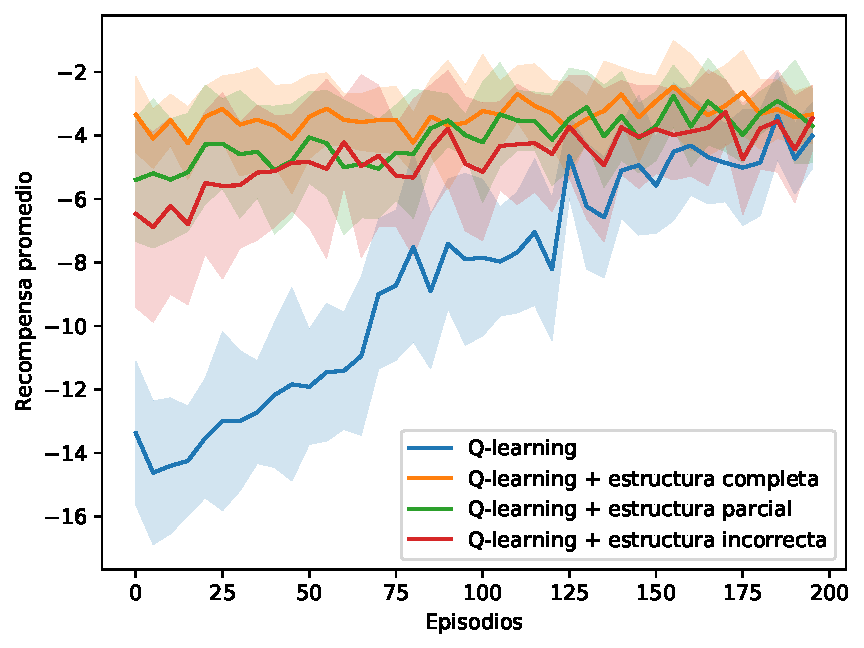
\includegraphics[width=.32\linewidth]{Chapter5/Figs/dqn/deterministic_low_025_many_to_one_N_9_experiments_10_episodes_200_eps_75.pdf}

\end{tabular}
\caption{Comparación del desempeño para los 4 algoritmos con $p_{mod} = 25 \%$ y $\delta = 75$ en un ambiente determinista y continuo. Las gráficas muestran la medida $average$ y la desviación estándar (región sombreada) para 10 experimentos con 200 episodios}
\label{fig:dqn-results-det}
\end{figure}

\newpage


\begin{figure}
\settoheight{\tempdima}{\includegraphics[width=.32\linewidth]{example-image-a}}%
\centering\begin{tabular}{@{}c@{ }c@{ }c@{ }c@{}}
&\textbf{Uno-a-uno} & \textbf{Causa común} & \textbf{Efecto común} \\
\rowname{$N = 5$}&
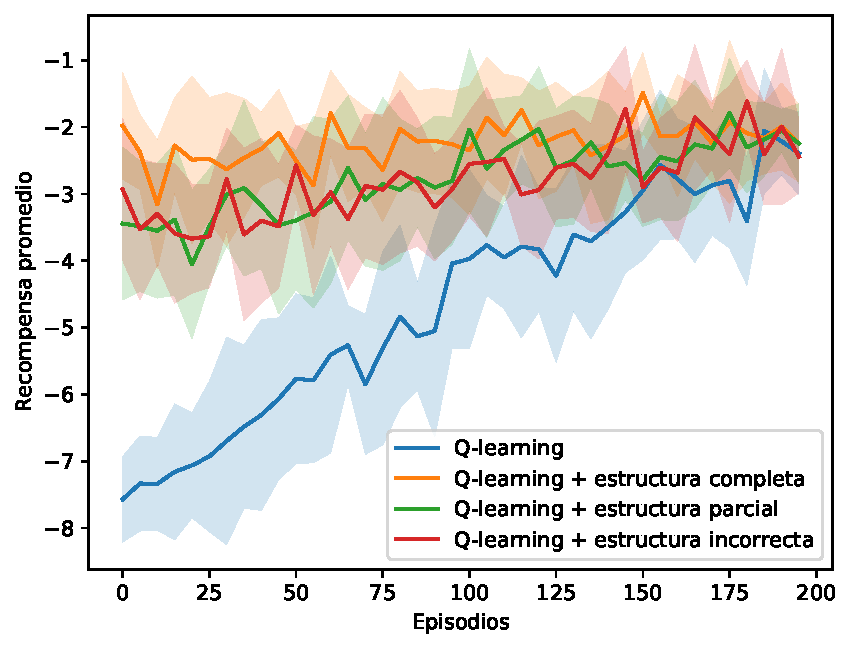
\includegraphics[width=.32\linewidth]{Chapter5/Figs/dqn/stochastic_low_025_one_to_one_N_5_experiments_10_episodes_200_eps_75.pdf}&
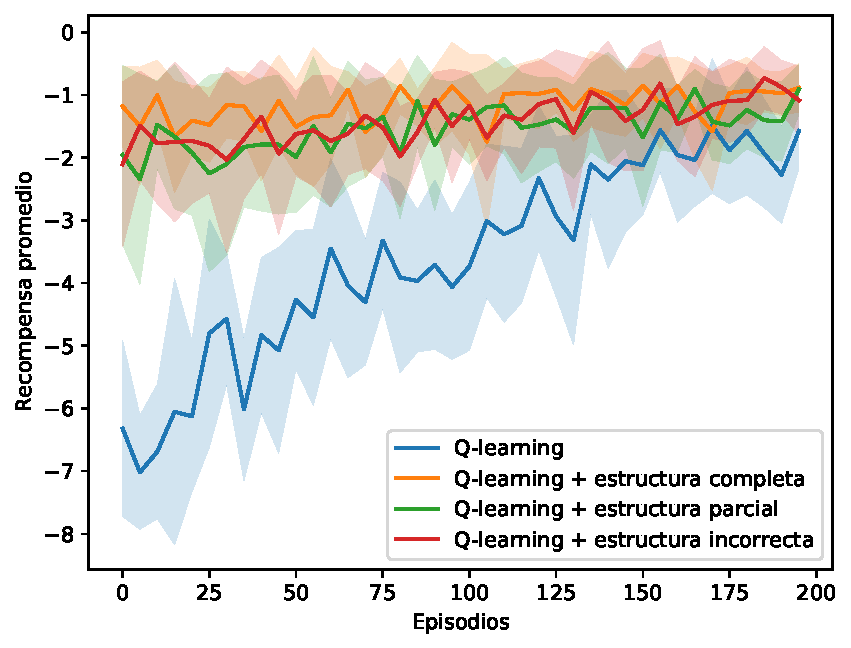
\includegraphics[width=.32\linewidth]{Chapter5/Figs/dqn/stochastic_low_025_one_to_many_N_5_experiments_10_episodes_200_eps_75.pdf}&
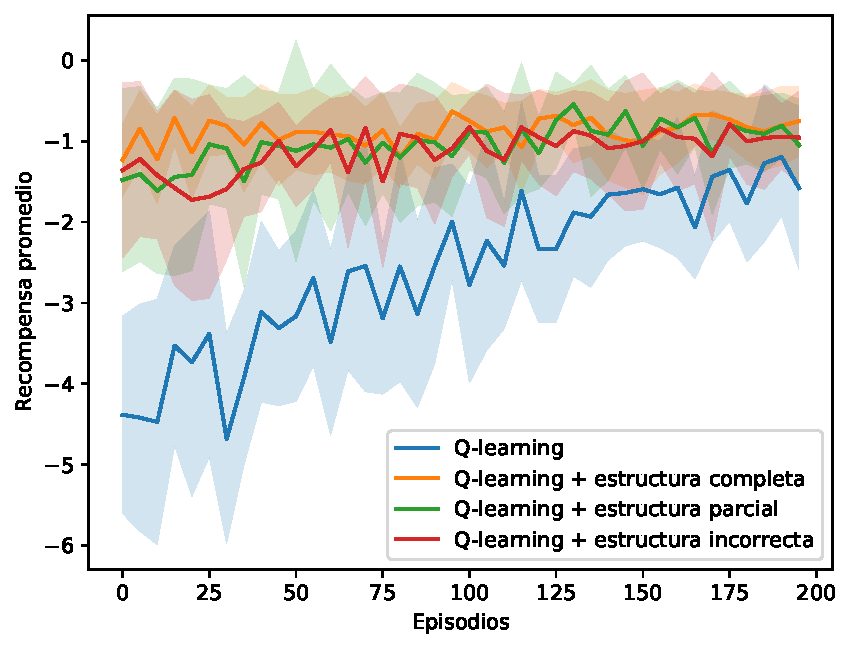
\includegraphics[width=.32\linewidth]{Chapter5/Figs/dqn/stochastic_low_025_many_to_one_N_5_experiments_10_episodes_200_eps_75.pdf}\\
\rowname{$N=7$}&
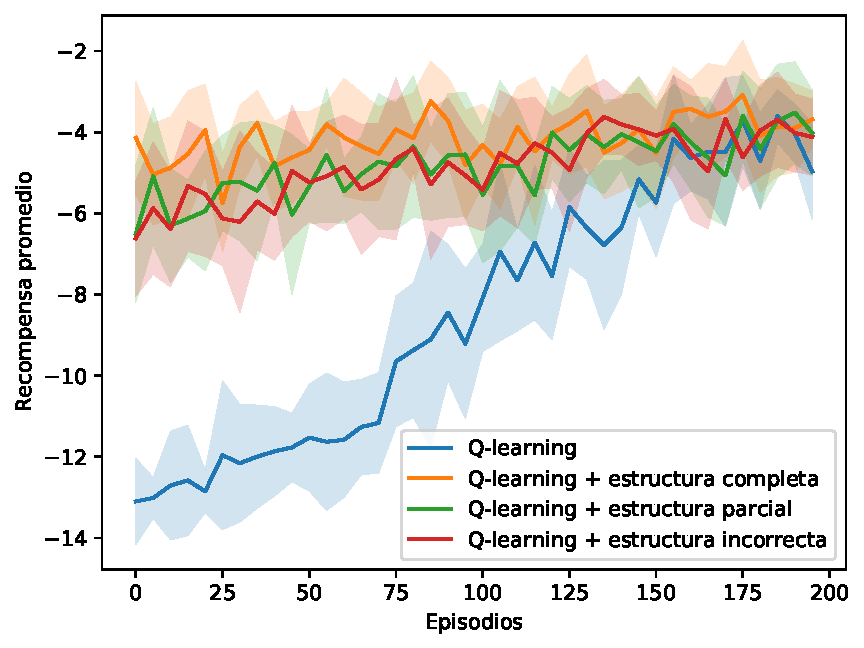
\includegraphics[width=.32\linewidth]{Chapter5/Figs/dqn/stochastic_low_025_one_to_one_N_7_experiments_10_episodes_200_eps_75.pdf}&
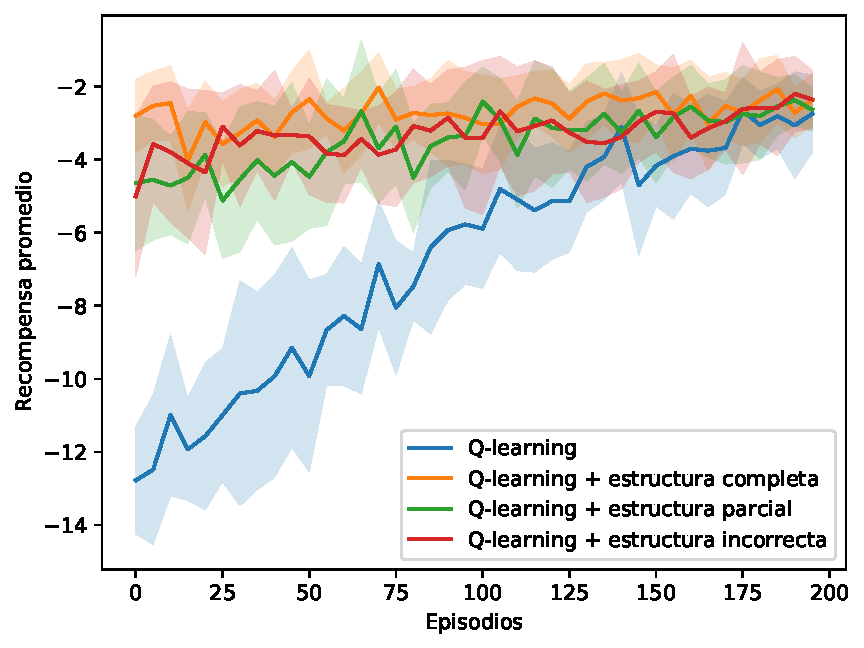
\includegraphics[width=.32\linewidth]{Chapter5/Figs/dqn/stochastic_low_025_one_to_many_N_7_experiments_10_episodes_200_eps_75.pdf}&
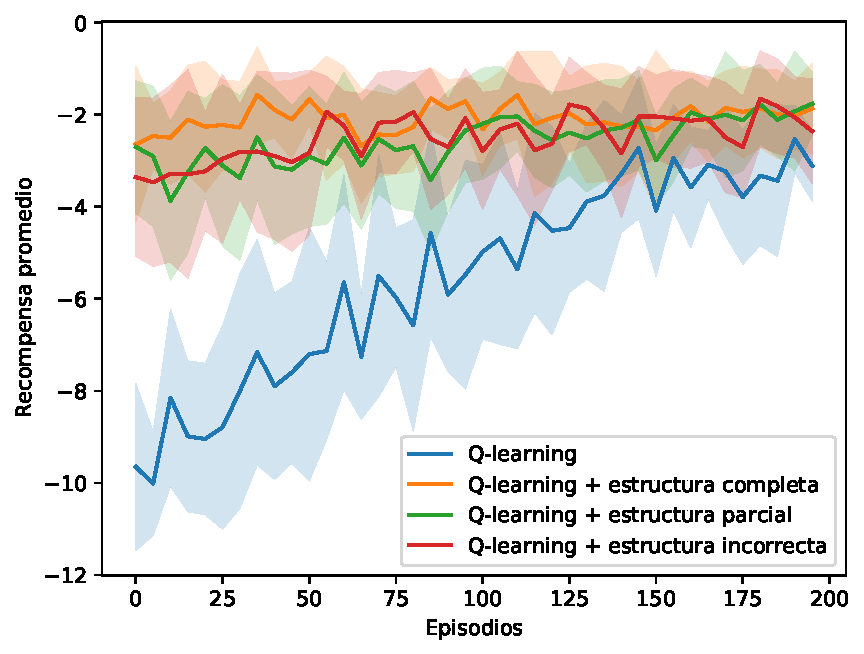
\includegraphics[width=.32\linewidth]{Chapter5/Figs/dqn/stochastic_low_025_many_to_one_N_7_experiments_10_episodes_200_eps_75.pdf}\\
\rowname{$N = 9$}&
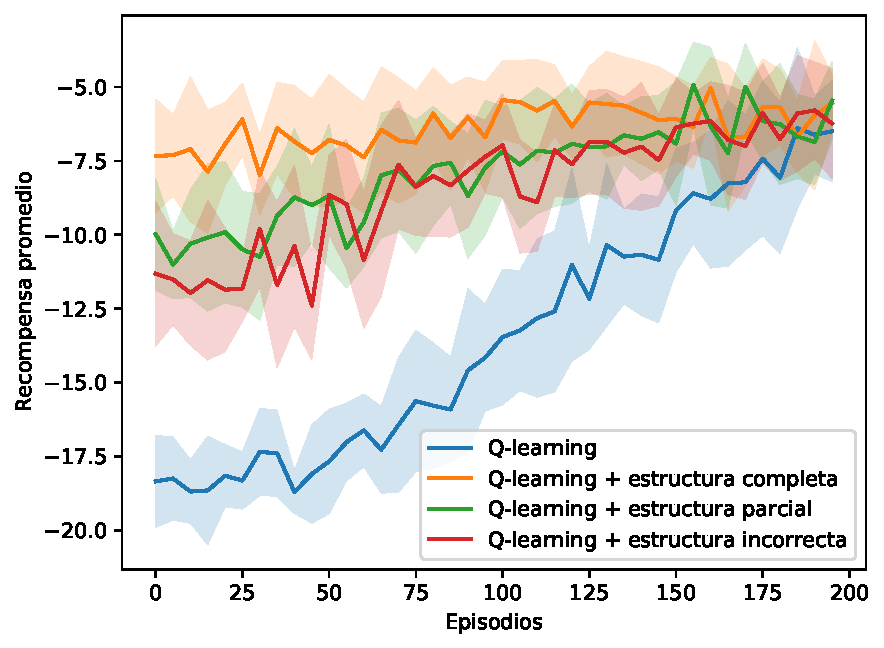
\includegraphics[width=.32\linewidth]{Chapter5/Figs/dqn/stochastic_low_025_one_to_one_N_9_experiments_10_episodes_200_eps_75.pdf}&
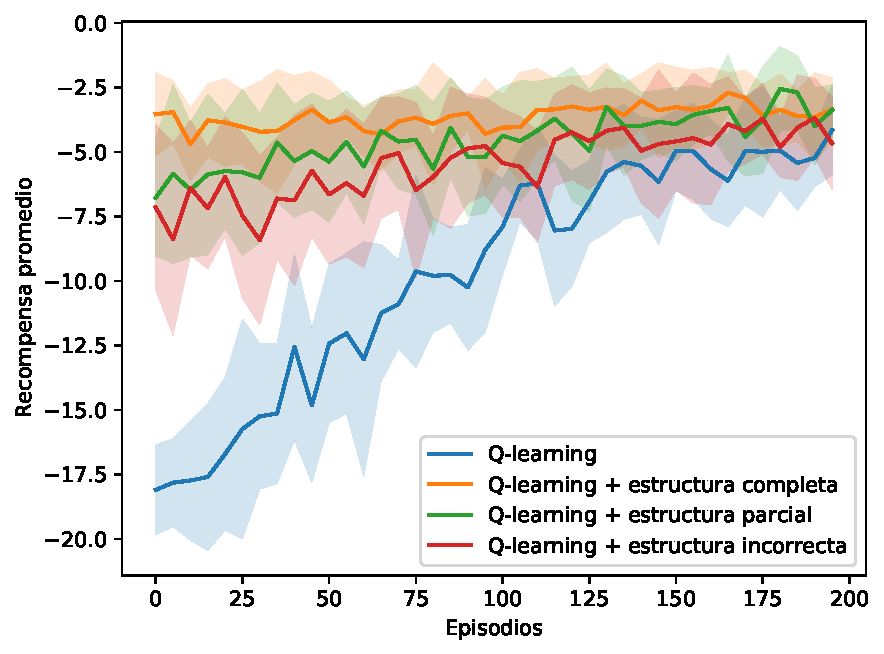
\includegraphics[width=.32\linewidth]{Chapter5/Figs/dqn/stochastic_low_025_one_to_many_N_9_experiments_10_episodes_200_eps_75.pdf}&
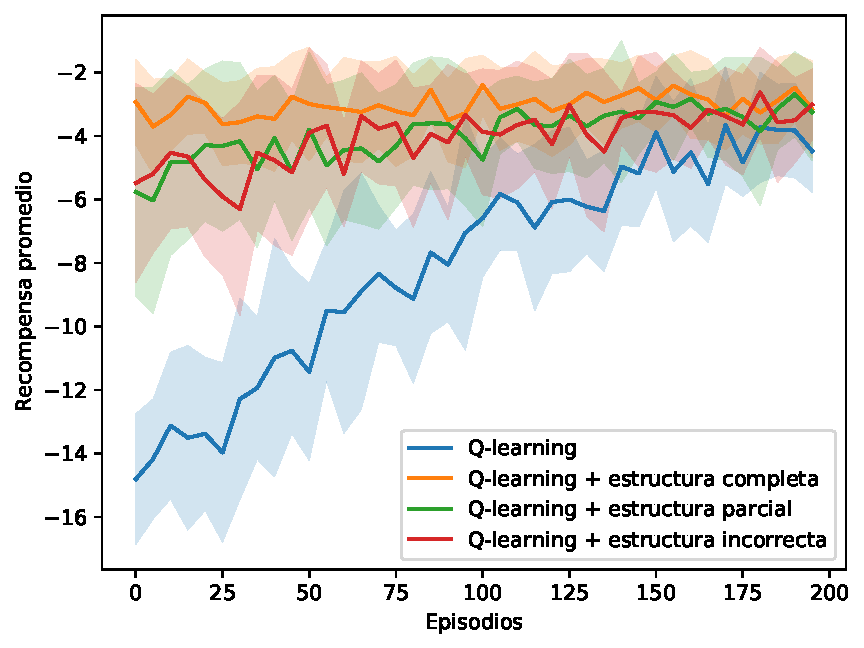
\includegraphics[width=.32\linewidth]{Chapter5/Figs/dqn/stochastic_low_025_many_to_one_N_9_experiments_10_episodes_200_eps_75.pdf}

\end{tabular}
\caption{Comparación del desempeño para los 4 algoritmos con $p_{mod} = 25 \%$ y $\delta = 75$ en un ambiente estocástico y continuo. Las gráficas muestran la medida $average$ y la desviación estándar (región sombreada) para 10 experimentos con 200 episodios}
\label{fig:dqn-results-sto}
\end{figure}
